\documentclass[
  bibliography=totoc,     % Literatur im Inhaltsverzeichnis
  captions=tableheading,  % Tabellenüberschriften
  titlepage=firstiscover, % Titelseite ist Deckblatt
]{scrartcl}

% Paket float verbessern
\usepackage{scrhack}

% Warnung, falls nochmal kompiliert werden muss
\usepackage[aux]{rerunfilecheck}

% unverzichtbare Mathe-Befehle
\usepackage{amsmath}
% viele Mathe-Symbole
\usepackage{amssymb}
% Erweiterungen für amsmath
\usepackage{mathtools}

% Fonteinstellungen
\usepackage{fontspec}

% Font Vorgaben:
\setmainfont{Arial}
\newfontfamily\arialfamily{Arial}
\addtokomafont{disposition}{\arialfamily}
% make sure Microsoft Fonts are installed
% on WSL you can just link the Windows Fonts directory in the Ubuntu Fonts directory
% https://www.hunterwebs.com.au/blog/how-to-sync-windows-fonts-with-wsl-windows-subsystem-for-linux/
% command for this: ln -s /mnt/c/windows/fonts ~/.fonts

% Zeilenabstand Vorgabe
\usepackage[onehalfspacing]{setspace}

% Wenn man andere Schriftarten gesetzt hat,
% sollte man das Seiten-Layout neu berechnen lassen
\recalctypearea{}

% deutsche Spracheinstellungen
\usepackage[ngerman]{babel}


\usepackage[
  math-style=ISO,    % ┐
  bold-style=ISO,    % │
  sans-style=italic, % │ ISO-Standard folgen
  nabla=upright,     % │
  partial=upright,   % ┘
  warnings-off={           % ┐
    mathtools-colon,       % │ unnötige Warnungen ausschalten
    mathtools-overbracket, % │
  },                       % ┘
]{unicode-math}

% traditionelle Fonts für Mathematik
\setmathfont{Latin Modern Math}
% Alternativ zum Beispiel:
%\setmathfont{Libertinus Math}

\setmathfont{XITS Math}[range={scr, bfscr}]
\setmathfont{XITS Math}[range={cal, bfcal}, StylisticSet=1]

% Zahlen und Einheiten
\usepackage[
  locale=DE,                   % deutsche Einstellungen
  separate-uncertainty=true,   % immer Unsicherheit mit \pm
  per-mode=symbol-or-fraction, % / in inline math, fraction in display math
]{siunitx}

% richtige Anführungszeichen
\usepackage[autostyle]{csquotes}

% Standardplatzierung für Floats einstellen
\usepackage{float}
\floatplacement{figure}{htbp}
\floatplacement{table}{htbp}

% figures in text
% https://en.wikibooks.org/wiki/LaTeX/Floats,_Figures_and_Captions#Wrapping_text_around_figures
\usepackage{wrapfig}

% Floats innerhalb einer Section halten
\usepackage[
  section, % Floats innerhalb der Section halten
  %below,   % unterhalb der Section aber auf der selben Seite ist ok
]{placeins}

% Seite drehen für breite Tabellen: landscape Umgebung
\usepackage{pdflscape}

% Captions schöner machen.
\usepackage[
  labelfont=bf,        % Tabelle x: Abbildung y: ist jetzt fett
  font=small,          % Schrift etwas kleiner als Dokument
  width=0.9\textwidth, % maximale Breite einer Caption schmaler
]{caption}

% subfigure, subtable, subref
\usepackage{subcaption}

% Grafiken können eingebunden werden
\usepackage{graphicx}

% schöne Tabellen
\usepackage{booktabs}

% Verbesserungen am Schriftbild
\usepackage{microtype}

% Literaturverzeichnis
\usepackage[
  backend=biber,
]{biblatex}

% Hyperlinks im Dokument
\usepackage[
  german,
  unicode,        % Unicode in PDF-Attributen erlauben
  pdfusetitle,    % Titel, Autoren und Datum als PDF-Attribute
  pdfcreator={},  % ┐ PDF-Attribute säubern
  pdfproducer={}, % ┘
]{hyperref}

% erweiterte Bookmarks im PDF
\usepackage{bookmark}

% Trennung von Wörtern mit Strichen
\usepackage[shortcuts]{extdash}

% Quellendatenbank
\addbibresource{bib/lit.bib}
\addbibresource{bib/programme.bib}

\author{%
  Nico Guth\\%
  \href{mailto:nico.guth@tu-dortmund.de}{nico.guth@tu-dortmund.de}%
}
\publishers{TU Dortmund – Fakultät Physik}

\subject{Maschinelles Lernen für Physiker}
\title{Projektbericht}
\subtitle{Segmentierung von Gewässern auf Satellitenbildern}
\date{Abgabe: 15.08.2021}

\begin{document}

\maketitle
\thispagestyle{empty}
\tableofcontents
\newpage

\section{Einleitung und Zielsetzung}
\label{sec:Einleitung}

Schon lange ist die Kartografie ein wesentlicher Teil des menschlichen Fortschritts.
Gegen Ende des 20. Jahrhunderts bis jetzt gewann die Kartografie anhand von Satellitenbildern zunehmender Wichtigkeit.
Dadurch hatten und haben Kartografen einen deutlich geringeren Aufwand große Gebiete der Erde abzudecken.
Da allerdings die zu kartografierende Fläche auf der Erde sehr groß ist, scheint eine vollständig manuelle Kartografie nicht mehr sinnvoll zu sein.
Ein zusätzliches Problem ist, dass Karten durchgehend angepasst werden müssen, da sich die Welt kontinuierlich verändert, 
sowohl durch menschliches Einwirken als auch durch natürliche Phänomene.

Um das Erstellen von Karten deutlich zu beschleunigen, wird seit einigen Jahren die Analyse der Satellitenbildern hauptsächlich von Computern durchgeführt.
Hierfür eignet sich maschinelles Lernen und insbesondere das \enquote{Deep Learning} mit Neuronalen Netzwerken.
Aber auch wenn heutzutage große Konzerne wie Google, Apple oder Microsoft schon sehr gute Algorithmen entwickelt haben,
ist es immernoch deulich zu erkennen, dass auch diese Algorithmen noch Fehler machen.

Deswegen ist Ziel dieses Projektes die Erkennung von Gewässern auf Satellitenbildern.
Genauer gesagt wird mithilfe von maschinellem Lernen zu jedem Eingangsbild eine Maske erzeugt, die jedem Pixel entweder Wasser oder kein Wasser zuordnet.
Außerdem werden nur Satellitenbilder innerhalb europäischer Länder und auf einer bestimmten Zoomstufe betrachtet.
Dadurch können nur größere Gewässer, also Seen, Flüsse oder das Meer erkannt werden und kleinere Gewässer wie Bäche, Teiche oder ähnliches sind nicht von großer Bedeutung für dieses Projekt.
Weitere Details zum Datensatz sind in \autoref{sec:Datensatz} erläutert.

Das Projekt ist Teil des Seminars \enquote{Maschinelles Lernen für Physiker} im Sommersemester 2021 und wurde von Samuel Haefs und mir (Nico Guth) durchgeführt.

\section{Datensatz}
\label{sec:Datensatz}

Da kein passender Datensatz gefunden wurde, musste dieser auch als Teil des Projekts erstellt werden.
Das Ziel war es für viele verschiedene Orte innerhalb europäischer Grenzen ein Satellitenbild und eine passende Maske zu haben.
Die Maske soll dabei die Pixel markieren, die zu größeren Wasserflächen wie Seen, Teichen, Flüssen, Kanälen oder Küsten vom Meer gehören.
Zusätzlich werden zu jedem Ort einige Metadaten wie die Koordinaten und das zugehörige Land gespeichert.
Ein Beispiel vom erzeugten Datensatz ist in \autoref{fig:datensatz_beispiel} zu sehen.

\begin{figure}
    \centering
    \begin{subfigure}{0.3\textwidth}
        \centering
        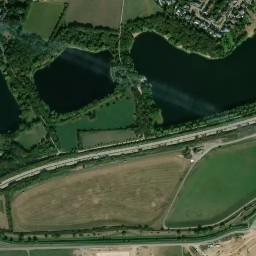
\includegraphics[width=\textwidth]{images/datensatz_beispiel_satellit.jpg}
        \caption{Satellitenbild}
        \label{fig:datensatz_beispiel_satellit}
    \end{subfigure}
    \begin{subfigure}{0.3\textwidth}
        \centering
        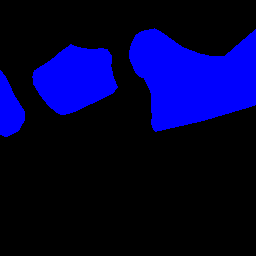
\includegraphics[width=\textwidth]{images/datensatz_beispiel_maske.png}
        \caption{Maskenbild}
        \label{fig:datensatz_beispiel_maske.png}
    \end{subfigure}
    \caption{\\Beispiel des Datensatzes an den Koordinaten %
            ${x_\text{Tile} = 16998}$, ${y_\text{Tile} = 10927}$, ${z_\text{Tile} = 15}$, %
            ${x_\text{Geo} = 6,751°}$, ${y_\text{Geo} = 51,293°}$. %
            (in Deutschland) \\ \copyright Mapbox, \copyright OpenStreetMap}
    \label{fig:datensatz_beispiel}
\end{figure}

Die Datensatz-Erstellung wurde mit Python automatisiert.
Im Folgenden soll auf die Vorgensweise eingegangen werden.

Die Daten wurden nicht in einer Sitzung sondern immer in kleinen Paketen gesammelt.
Zuerst wurden gleichverteilte Zufallszahlen für Längengrad $x_\text{Geo}$ und Breitengrad $y_\text{Geo}$ (also in geographischen Koordinaten) 
im Bereich $x_\text{Geo} \in [-10,49° \,,\, 40,27°]$, $y_\text{Geo} \in [34,51° \,,\, 71,20°]$ gezogen.
Dieser Bereich ist eine grobe Begrenzung für Europa.
Für jeden so gezogenen Ort wurde mithilfe der groben Ländergrenzen des \enquote{Natural Earth Data} Projektes überprüft, 
ob dieser Ort innerhalb eines europäischen Landes liegt. \cite{natural_earth_countries}
Allerdings wurden Russland und Island nicht miteinbezogen.

Ziel war es viele Satellitenbilder zu sammeln, die Wasser enthalten.
Da in Europa allerdings das Verhältnis von Wasser- zu Landfläche sehr gering ist, musste vor dem Herunterladen der Wassergehalt des Bildes überprüft werden.
Dies wurde mithilfe der Daten der \enquote{Mapbox Vector Tiles API} überprüft. \cite{mapbox_vector_tiles}
Ein Ort wurde nur dann akzeptiert, wenn dieser nicht doppelt gezogen wurde und das Bild nicht gar kein, aber auch nicht nur Wasser enthält.

Für jeden akzeptierten Ort wurde dann mithilfe der \enquote{Mapbox Raster Tiles API} ein Satellitenbild heruntergeladen.\cite{mapbox_raster_tiles}
Außerdem wurde mithilfe der \enquote{Mapbox Static Tiles API} und einem selbst angepassten Kartenstil von diesem Ort ein Maskenbild für den Wassergehalt heruntergeladen.\cite{mapbox_static_tiles}
Mapbox verwendet für die Kartendaten \enquote{OpenStreetMap} und somit stammen auch die Daten der Maskenbilder daher.\cite{OpenStreetMap}

An dieser Stelle scheint es sinnvoll zu erwähnen, dass die Maskenbilder teilweise Fehler enthalten und Gewässer nur sehr grob oder auch falsch zugeordnet sind. 

In der Bereitstellung von digitalen Karten und geographischen Daten wird heutzutage vermehrt das Konzept sogenannter \enquote{Tiles} verwendet.\cite{tiles}
Hier ist eine Zoom-Stufe $z_\text{Tile}$ anzugeben und die Welt wird in $4^{z_\text{Tile}}$ gleichgroße Quadrate(\enquote{Tiles}) aufgeteilt.
Jedem dieser Quadrate wird eine $x_\text{Tile}$- und eine $y_\text{Tile}$-Koordinate zugeordnet.

Während der Erstellung des Datensatzes musste zwischen einigen Koordinatensystemen gewechselt werden, aber die Koordinaten der \enquote{Tiles} waren ausschlaggebend für die heruntergeladenen Bilder.
Jedes Bild im Datensatz wurde mit einer Zoom-Stufe $z_\text{Tile} = 15$ generiert und entspricht genau einem \enquote{Tile}.

Der Datensatz enthielt am Ende des Projektes 57931 Satellitenbilder und dazu passende Maskenbilder.
Jedes Bild hatte eine Auflösung von 256 x 256 Pixel.

\section{Vorgehensweise}
\label{sec:Vorgehensweise}

Ziel dieses Projektes war es Wasser auf Satellitenbildern zu erkennen.
Dazu wurden zwei Methoden des maschinellen Lernens für die Segmentierung verwendet.
Ein \enquote{Convolutional Neural Network} stellte dabei die Hauptmethode dar 
und ein \enquote{Random Forest} stellte dabei eine Alternativmethode zum Vergleich dar.
Für beide Methoden wurde das Framework \enquote{TensorFlow} verwendet.\cite{tensorflow}
Die Metrik, die benutzt wurde um die Methoden zu evaluieren, war die Genauigkeit(zu englisch \enquote{accuracy}), 
also der Anteil der richtig zugeordneten Pixel.

\subsection{Vorverarbeitung}
\label{ssec:Vorverarbeitung}

Der in \autoref{sec:Datensatz} beschriebene Datensatz wurde in drei Teildatensätze aufgeteilt,
den Trainings-, den Validierungs- und den Testdatensatz.
Die Größen dieser Datensätze sind in \autoref{tab:Teildatensätze} angegeben.

\begin{table}
    \centering
    \caption{Größen der Teildatensätze vom Gesamtdatensatz mit 57931 Satellitenbildern.}
    \label{tab:Teildatensätze}
    \begin{tabular}{l c c c}
        \toprule 
        & Trainingsdaten & Validierungsdaten & Testdaten \\ 
        \midrule 
        Anzahl & 39392 & 6952 & 11587 \\
        Anteil & 68\% & 12\% & 20\% \\
        \bottomrule
    \end{tabular}
\end{table}

Außerdem wurden die Bilder zu einer Auflösung von 128 x 128 Pixel skaliert, 
da so nicht viel Information verloren ging und viel Rechenzeit und Rechenleistung eingespart werden konnte.
Die Pixel der Maskenbilder wurden zu binären Werten umgerechnet, wobei 1 Wasser und 0 kein Wasser kennzeichnet
und die drei Farbkanäle Satellitenbilder wurden auf einen Pixelwert zwischen 0 und 1 normiert. 

\subsection{Hauptmethode: \enquote{Convolutional Neural Network}}
\label{ssec:Hauptmethode}

Das verwendete Neuronale Netzwerk ist vollständig \enquote{convolutional} und orientiert sich an der häufig für Segmentierung verwendeten \enquote{U-Net}-Struktur.\cite{ronneberger2015unet}
Hier wird in der ersten Hälfte des Netzwerks zwischen den \enquote{convolutional} Lagen das Bild in durch maximales \enquote{Pooling} verkleinert (halbierte Kantenlänge) 
und in der zweiten Hälfte das Bild zwischen den \enquote{convolutional} Lagen durch transponierte \enquote{convolutional} Lagen vergrößert (verdoppelte Kantenlänge).
Zusätzlich wird die Ausgabe vor dem Verkleinern kopiert und mit der Ausgabe nach dem Vergrößern verkettet.
Ein Beispiel eines solchen \enquote{U-Net} ist in \autoref{fig:unet} dargestellt.
Außerdem wurde zwischen den beiden \enquote{convolutional} Lagen einer Ebene das Netzwerk mithilfe von \enquote{Dropout} regularisiert.
Ein weiterer Unterschied zum dargestellten \enquote{U-Net} ist, dass bei den \enquote{convolutional} Lagen ein \enquote{Padding} von \enquote{same} statt \enquote{valid} verwendet wurde.

Als Aktivierungsfunktion wurde für alle \enquote{convolutional} Lagen die \enquote{ReLU}-Funktion und für die letzte Lage die \enquote{Sigmoid}-Funktion verwendet.
Der Optimierer \enquote{Adam} hat dabei die Verlustfunktion der binären Kreuzentropie minimiert.

\begin{figure}
    \centering
    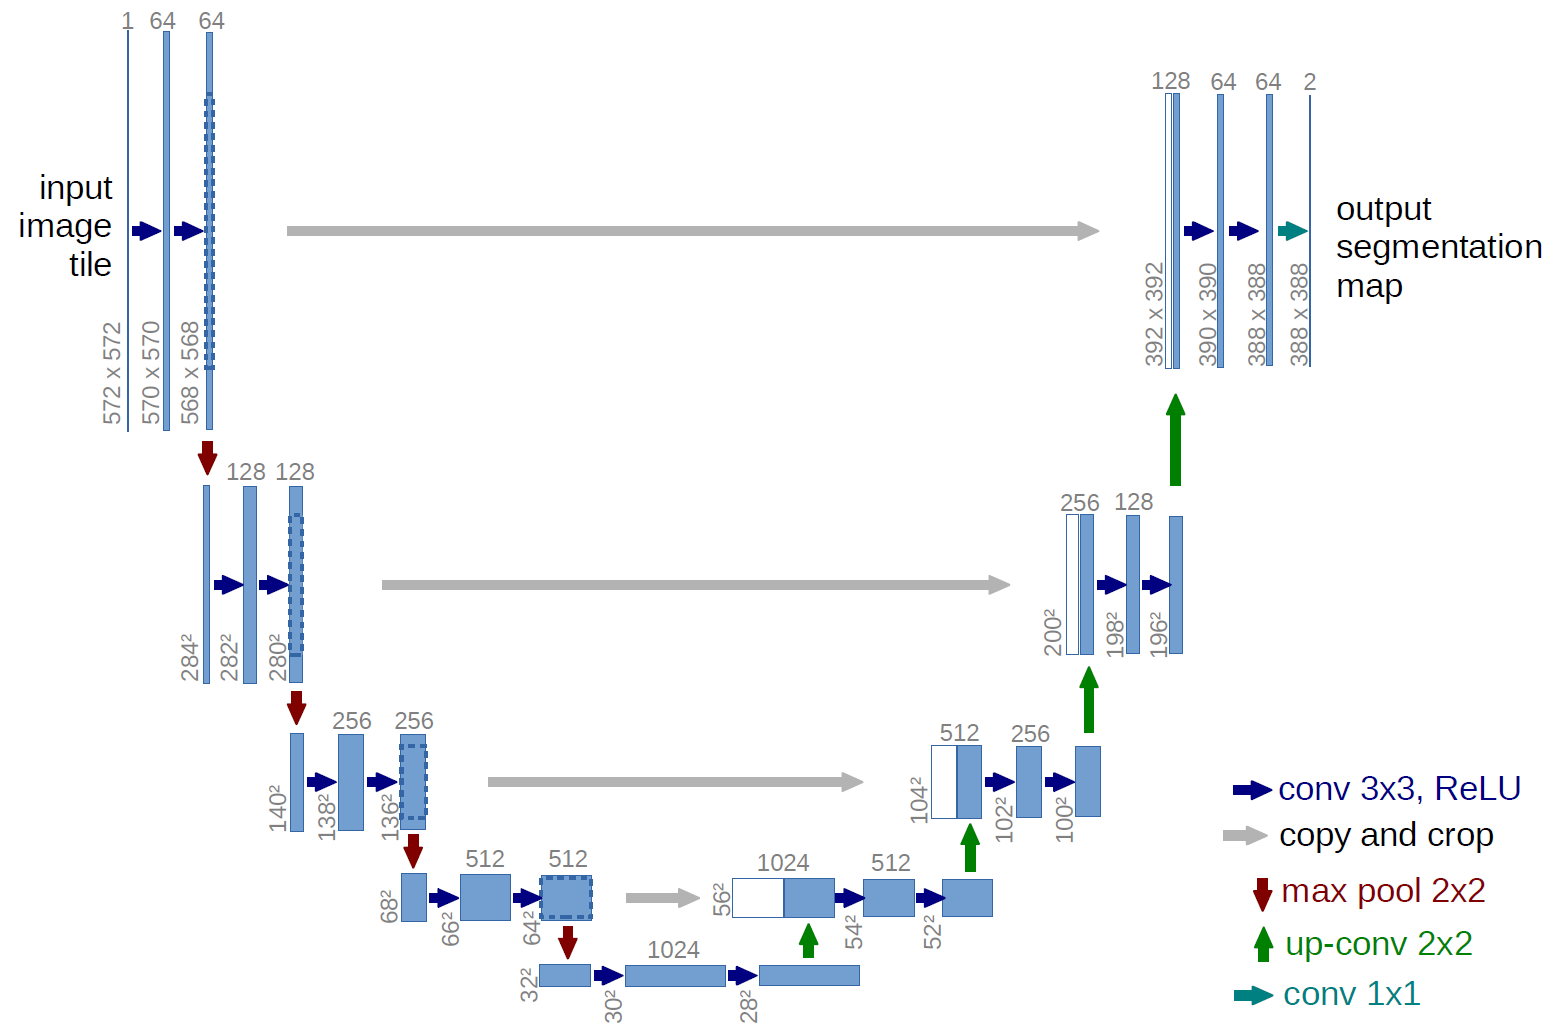
\includegraphics[width=0.6\textwidth]{images/unet.png}
    \caption{Visualisierung eines \enquote{U-Net}, %
    wobei jede Box einem Mehrkanal-Bild entspricht. Die Anzahl an Kanäle ist über der Box angegeben und die Anzahl der Pixel ist neben der Box angegeben. %
    Jeder Pfeil entspricht der entsprechenden Operation.\cite{ronneberger2015unet}}
    \label{fig:visual_model}
\end{figure}

Die besten Hyperparameter und die beste Struktur des Netzwerks wurde mithilfe einer zufälligen Suche ermittelt.
Das Netzwerk wurde für 100 verschiedene Kombinationen der Hyperparameter auf einem kleinen Trainingsdatensatz von 3000 Satellitenbildern trainiert
und dann auf einem kleinen Validierungsdatensatz von ebenfalls 3000 Satellitenbildern evaluiert.
Das Ergebnis der Hyperparametersuche ist in \autoref{fig:grid_search} dargestellt.
Variiert wurden folgende Hyperparameter:

\begin{itemize}
    \item \enquote{filter\_start}: Anzahl der Filter der \enquote{convolutional} Lagen der ersten und letzten Ebene, wobei die Filter pro Ebene verdoppelt wurden
    \item \enquote{filter\_levels}: Anzahl der Ebenen
    \item \enquote{kernel\_size}: Größe der Faltungsmatrizen aller \enquote{convolutional} Lagen
    \item \enquote{kernel\_initializer}: Methode der Matrixinitialisierung aller \enquote{convolutional} Lagen
    \item \enquote{dropout\_start}: Stärke des \enquote{Dropout} der ersten und letzten Ebene, wobei die Stärke jeweils nach zwei Ebenen um 0,1 erhöht wurde
    \item \enquote{learning\_rate}: Lernrate des verwendeten Optimierers \enquote{Adam}
\end{itemize}

\begin{figure}
    \centering
    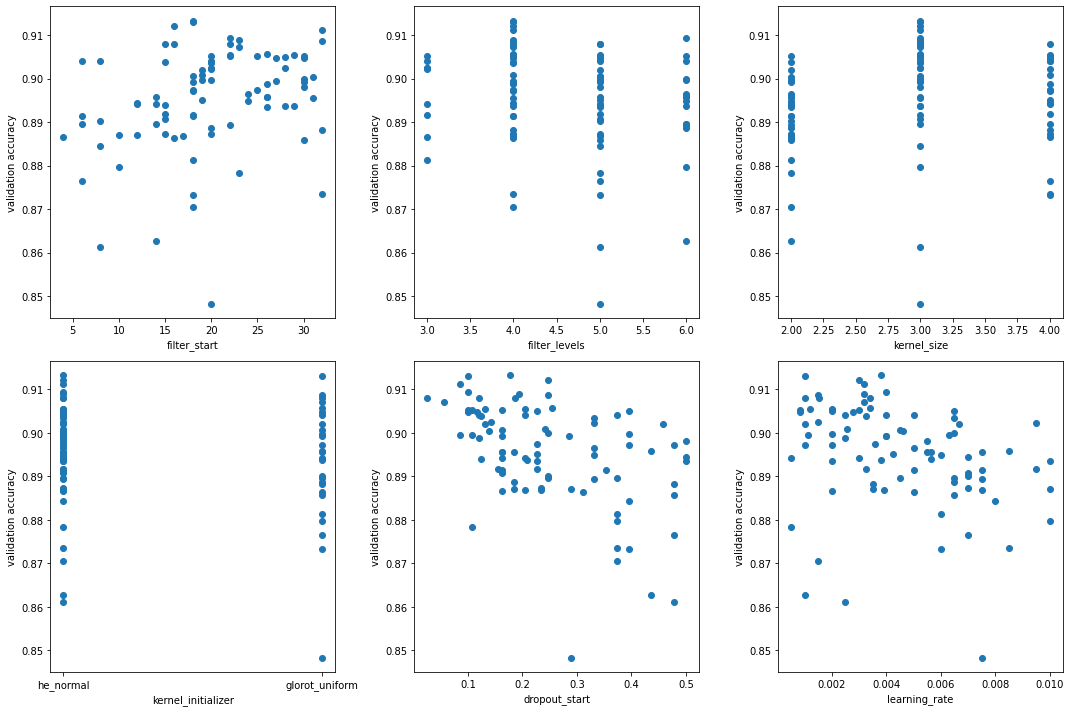
\includegraphics[width=0.8\textwidth]{images/grid_search.png}
    \caption{Zufällige Suche der besten Hyperparameter}
    \label{fig:grid_search}
\end{figure}

Vor dieser systematischen Suche wurden weitere Hyperparameter variiert, allerdings erwies sich das zuvor beschriebene Neuronale Netzwerk als am besten geeignet
und die systematischen Suche beschränkte sich auf die wichtigsten Parameter.

Aus der Suche ergab sich eine Kombination mit der besten Genauigkeit von 91,3\% auf dem Validierungsdatensatz.
Das dadurch entstandene Netzwerk wurde dann für den gesamten Datensatz verwendet und wird im Folgenden anhand der Visualisierung in \autoref{fig:visual_model} detailliert beschrieben.
Die Aufzählungen im Folgenden sind in \autoref{fig:visual_model} von links nach rechts der entsprechenden Lage zugeordnet.

\begin{figure}
    \centering
    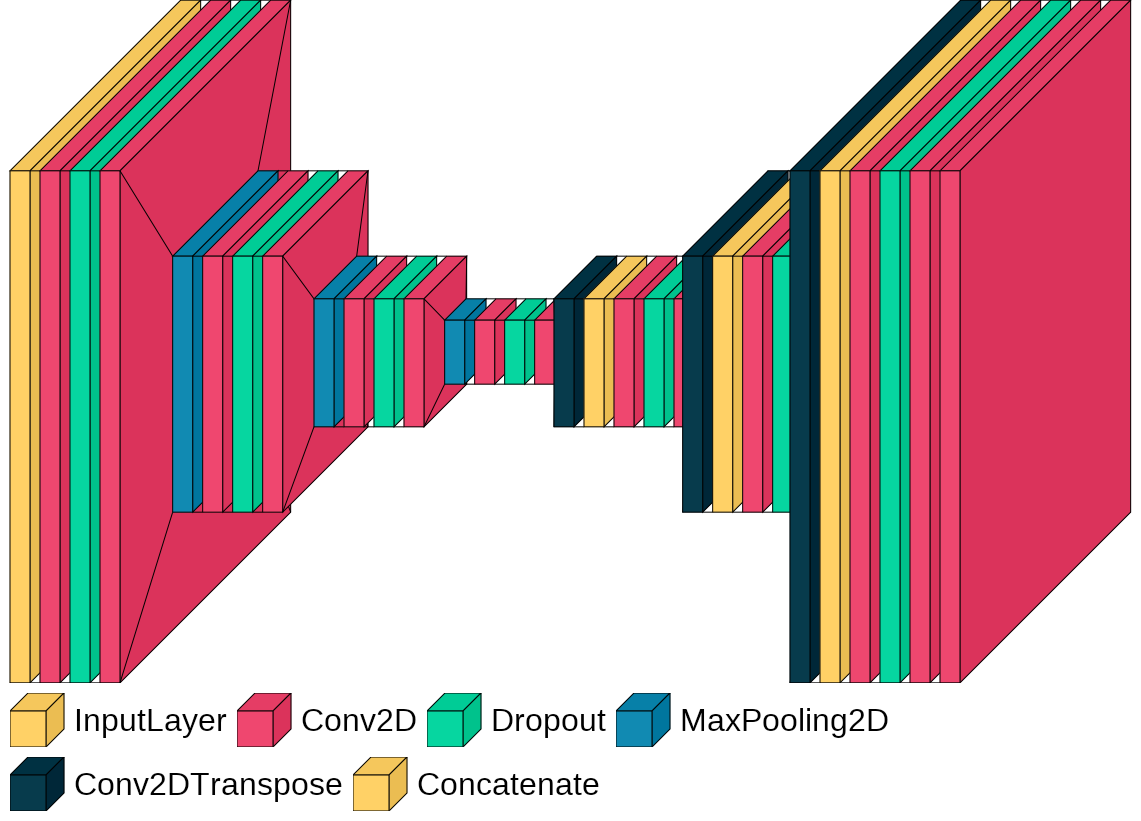
\includegraphics[width=0.6\textwidth]{images/visual_model.png}
    \caption{Visualisierung des verwendeten Convolutional Neural Network}
    \label{fig:visual_model}
\end{figure}

\begin{itemize}
    \item \enquote{InputLayer} Shape: (..., 128, 128, 3) 
    \item \enquote{Conv2D}:
    \item[-] Filter Anzahl: 18, 18, 36, 36, 72, 72, 144, 144, 72, 72, 36, 36, 18, 18, 1
    \item[-] Kernel Größe: 3 x 3
    \item[-] Kernel Initialisierungs-Methode: \enquote{he\_normal}
    \item[-] Padding: \enquote{same} 
    \item[-] Aktivierungsfunktion: ReLU (letzte: Sigmoid)
    \item \enquote{Dropout} Stärke: 0.1779, 0.1779, 0.2779, 0.2779, 0.2779, 0.1779, 0.1779
    \item \enquote{MaxPooling2D} Größe: 2 x 2
    \item \enquote{Conv2DTranspose}:
    \item[-] Filter Anzahl: 72, 36, 18
    \item[-] Kernel Größe: 2 x 2
    \item[-] Aktivierungsfunktion: keine
    \item \enquote{Concatenate}: Verkettet Ausgabe vor \enquote{MaxPooling2D} mit Ausgabe nach \enquote{Conv2DTranspose} der gleichen Ebene
    \item Verlustfunktion: binäre Kreuzentropie
    \item \enquote{Adam}-Lernrate: 0.003795
    \item \enquote{Batch}-Größe beim Training: 128
\end{itemize}

Der Fortschritt während des Trainings ist in \autoref{fig:train_hist} dargestellt.

\begin{figure}
    \centering
    \begin{subfigure}{0.45\textwidth}
        \centering
        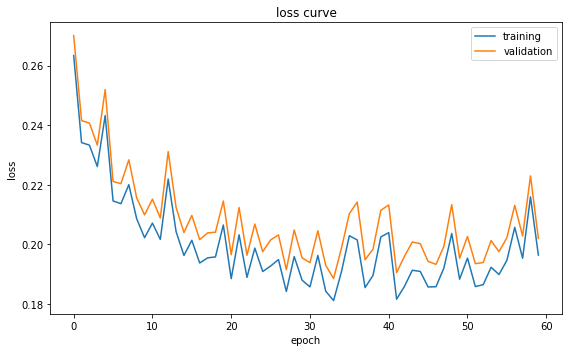
\includegraphics[width=\textwidth]{images/loss_curve.png}
        \caption{Verlustfunktion}
        \label{fig:loss_curve}
    \end{subfigure}
    \begin{subfigure}{0.45\textwidth}
        \centering
        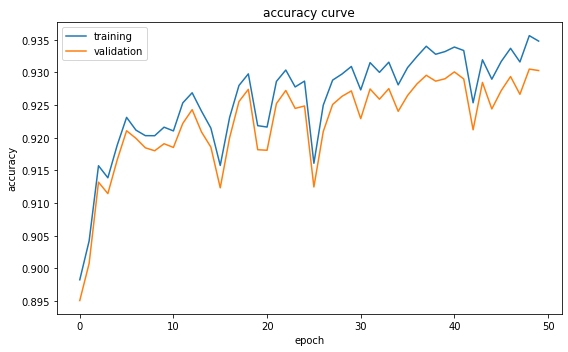
\includegraphics[width=\textwidth]{images/acc_curve.png}
        \caption{Genauigkeit}
        \label{fig:acc_curve}
    \end{subfigure}
    \caption{Plots der Verlustfunktion bzw. Genauigkeit während dem Training je nach Epoche auf Trainings- und Validierungsdatensatz}
    \label{fig:train_hist}
\end{figure}

Da die Pixel der Ausgabebilder des Netzwerks Werte zwischen 0 und 1 annimmt, wurde ein die Genauigkeit auf dem Validierungsdatensatz
für verschiedene Schwellwerte berechnet, ab denen ein Pixel als Wasser gewertet wird.
Dies ist in \label{fig:threshold} dargestellt.

\begin{figure}
    \centering
    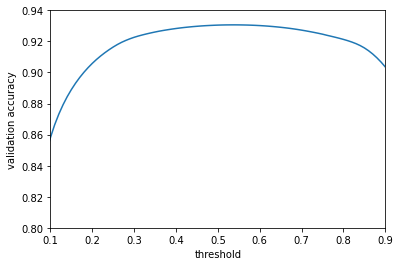
\includegraphics[0.5\textwidth]{images/threshold.png}
    \caption{Plot der Genauigkeit auf dem Validierungsdatensatz gegen den Schwellwert}
    \label{fig:threshold}
\end{figure}

\subsection{Alternativmethode: \enquote{Random Forest}}
\label{ssec:Alternativmethode}

Zum Vergleich mit dem Neuronalen Netzwerks wurde eine Pixelweise Klassifikation mithilfe eines \enquote{Random Forest} verwendet.
Auch hierfür wurde das Framework \enquote{TensorFlow} verwendet, allerdings wurde dies um das Framework \enquote{TensorFlow Decision Forests} erweitert.\cite{tfdf}
Dieser \enquote{Random Forest} besteht aus 60 Entscheidungsbäumen, die eine maximale Tiefe von 32 haben.

Hierfür wurden zunächst jedem Pixel der Satellitenbilder einige Attribute extrahiert.
Auf jedem Farbkanal wurde der Betrag des Gradienten berechnet.
Dann wurde vom Satellitenbild und dem Bild der Gradienten ein Graustufen Bild erzeugt.
All diese 8 Attribute wurden dem \enquote{Random Forest} pixelweise übergeben.

Aufgrund von Arbeitsspeicher- und Rechenzeit-Limitierungen konnte nicht der gesamte Trainingsdatensatz verwendet werden.
Aus jedem Bild im Trainingsdatensatz wurden 25 zufällige Pixel verwendet und so wurde der \enquote{Random Forest} auf einer Millionen Pixel trainiert.
Der Validierungs- und Testdatensatz blieb jedoch gleich.

\section{Ergebnisse}
\label{sec:Ergebnisse}

Lorem ipsum dolor sit amet, consetetur sadipscing elitr, sed diam nonumy eirmod tempor invidunt ut labore et dolore magna aliquyam erat, sed diam voluptua. At vero eos et accusam et justo duo dolores et ea rebum. Stet clita kasd gubergren, no sea takimata sanctus est Lorem ipsum dolor sit amet. Lorem ipsum dolor sit amet, consetetur sadipscing elitr, sed diam nonumy eirmod tempor invidunt ut labore et dolore magna aliquyam erat, sed diam voluptua. At vero eos et accusam et justo duo dolores et ea rebum. Stet clita kasd gubergren, no sea takimata sanctus est Lorem ipsum dolor sit amet. Lorem ipsum dolor sit amet, consetetur sadipscing elitr, sed diam nonumy eirmod tempor invidunt ut labore et dolore magna aliquyam erat, sed diam voluptua. At vero eos et accusam et justo duo dolores et ea rebum. Stet clita kasd gubergren, no sea takimata sanctus est Lorem ipsum dolor sit amet. 

Duis autem vel eum iriure dolor in hendrerit in vulputate velit esse molestie consequat, vel illum dolore eu feugiat nulla facilisis at vero eros et accumsan et iusto odio dignissim qui blandit praesent luptatum zzril delenit augue duis dolore te feugait nulla facilisi. Lorem ipsum dolor sit amet, consectetuer adipiscing elit, sed diam nonummy nibh euismod tincidunt ut laoreet dolore magna aliquam erat volutpat. 

Ut wisi enim ad minim veniam, quis nostrud exerci tation ullamcorper suscipit lobortis nisl ut aliquip ex ea commodo consequat. Duis autem vel eum iriure dolor in hendrerit in vulputate velit esse molestie consequat, vel illum dolore eu feugiat nulla facilisis at vero eros et accumsan et iusto odio dignissim qui blandit praesent luptatum zzril delenit augue duis dolore te feugait nulla facilisi. 

Nam liber tempor cum soluta nobis eleifend option congue nihil imperdiet doming id quod mazim placerat facer possim assum. Lorem ipsum dolor sit amet, consectetuer adipiscing elit, sed diam nonummy nibh euismod tincidunt ut laoreet dolore magna aliquam erat volutpat. Ut wisi enim ad minim veniam, quis nostrud exerci tation ullamcorper suscipit lobortis nisl ut aliquip ex ea commodo consequat. 

Duis autem vel eum iriure dolor in hendrerit in vulputate velit esse molestie consequat, vel illum dolore eu feugiat nulla facilisis. 

\section{Fazit}
\label{sec:Fazit}

Die Ergebnisse beider verwendeten Methoden zur Segmentierung von Gewässern auf Satellitenbildern waren ausreichend
und übertrafen teilweise unsere Erwartungen vor dem Projekt.
Erst während des Projektes erkannten wir, dass einige der Masken im Datensatz fehlerhaft waren.
Auch erkannten wir, dass ein paar der Satellitenbilder für eine Segmentierung unbrauchbar waren. (z.B. Bilder von Wolken)
Trotz der schlechten Daten, die zum Training verwendet wurden, wurden gute Ergebnisse erzielt 
und die vorhergesagten Masken waren häufig besser als die Masken des Datensatzes.
Die erzielten Genauigkeiten der Hauptmethode von etwa 93\% und der Alternativmethode von etwa 89\% lassen sich allerdings nicht näher beurteilen, 
da nicht klar ist welche Genauigkeit die Masken im Datensatz erreichen und diese Masken als Grundwahrheit angenommen wurden.
Hierfür wäre eine manuelle Überprüfung notwendig.

Der Vergleich des Convolutional Neural Network zum Random Forest zeigte deutlich, dass für dieses Problem ersteres besser geeignet war.
Zusätzlich zu den besseren Ergebnissen war das Convolutional Neural Network deutlich sparsamer mit der benötigten Rechenleistung 
und sogar die Vorhersagen wurden deutlich schneller erzeugt als bei dem Random Forest.
Auch ist zu sehen, dass das Convolutional Neural Network Beziehungen zwischen den Pixeln auswertete, was bei dem Random Forest nicht möglich war.

Durch eine ausführlichere Hyperparametersuche könnte das Modell weiter optimiert werden. 
Es wurde allerdings gezeigt, dass ein so komplexes und vielseitiges Problem 
wie die Wassererkennung auf Satellitenbildern mit Deep Learning gelöst werden kann.
Eine Überwachung der Ausgabe von neuronalen Netzen durch Menschen ist allerdings noch zu empfehlen.

Abschließend sei zu sagen, dass dieses Projekt uns den Umgang mit Deep Learning weiter nahegebracht hat 
und gezeigt hat wie vielseitig einsetzbar neuronale Netzwerke sind.


\printbibliography{}

\end{document}
